\documentclass[10pt]{article}

% Idioma y codificación
\usepackage[utf8]{inputenc}
\usepackage[spanish]{babel}

% Márgenes
\usepackage{geometry}
\geometry{top=2.5cm, bottom=2.5cm, left=2.5cm, right=2.5cm}

% Gráficos
\usepackage{graphicx}
\usepackage{graphics}
\usepackage{wrapfig}
\usepackage{float}

% Listings para código
\usepackage{listings}
\usepackage{xcolor}
\usepackage{caption}
\usepackage{capt-of}
\lstdefinestyle{terminal}{
	backgroundcolor=\color{gray!10},
	basicstyle=\ttfamily\small,
	keywordstyle=\color{blue},
	commentstyle=\color{gray},
	frame=single,
	columns=fullflexible,
	morecomment=[l]{//}
}
\usepackage{listings}
\lstset{
	inputencoding=utf8,
	extendedchars=true,
	literate={á}{{\'a}}1 {é}{{\'e}}1 {í}{{\'i}}1 {ó}{{\'o}}1 {ú}{{\'u}}1 {ñ}{{\~n}}1
}

% Hipervínculos
\usepackage[hidelinks]{hyperref}
\hypersetup{
	colorlinks=true,
	linkcolor=blue,
	filecolor=magenta,
	urlcolor=cyan,
}

\usepackage{url}

% Encabezados y pies de página
\usepackage{fancyhdr}
\pagestyle{fancy}
\fancyhf{}
\fancyfoot[R]{\thepage}

% Formato de títulos
\usepackage{titlesec}
\titleformat{\subsection}{\normalfont\large\bfseries}{\hspace{1em}\thesubsection}{1em}{}
\titleformat{\subsubsection}{\normalfont\normalsize\bfseries}{\hspace{2em}\thesubsubsection}{1em}{}

% Datos de la portada
\title{\textbf{Cuaderno de bitácora}}
\author{\textbf{\small Daniel Sanabria Salamanqués}}
\date{\today}

\makeatletter
\let\thetitle\@title
\let\theauthor\@author
\let\thedate\@date
\makeatother

\begin{document}
	
	\begin{titlepage}
		\centering
		\includegraphics[scale=0.3]{uva-3881270087.pdf}\\[0.5cm]
		\rule{\linewidth}{0.2mm}\\[0.4cm]
		{\huge\bfseries \thetitle}\\
		\rule{\linewidth}{0.2mm}\\[1.5cm]
		{\Large\bfseries Ingeniería Informática}\\[0.3cm]
		{\Large\bfseries Tecnologías de la Información}\\[1cm]
		{\Large \theauthor}\\[1.5cm]
		{\Large \thedate}
	\end{titlepage}
	
	\renewcommand{\contentsname}{Índice}
	\tableofcontents
	\clearpage
	\section{Instalación}
	
	\subsection{Clúster de Máquinas Virtuales}
	Para comenzar con la instalación, me dirijo a la página \url{matrix.inf.uva.es} e inicio sesión con mi cuenta de laboratorio de la escuela. Una vez hecho, observo que en el \verb|Datacenter| se encuentra mi máquina virtual \verb|vm3803.virtual.lab.inf.uva.es|. Al hacer doble clic, compruebo en la sección de \verb|Hardware| si está en el apartado \verb|CD/DVD| la imagen de \verb|Ubuntu Server|. Como no aparece, hago clic sobre ese apartado y con la opción \verb|Edit| que aparece en la parte superior, agrego la imagen a ese disco de la máquina.
	
	\subsection{Configuración de instalación}
	Tras esto, voy a la sección \verb|Console| para iniciar la máquina virtual y comenzar con la instalación de \verb|Ubuntu Server|. Lo primero es seleccionar el idioma para el sistema; en mi caso, escojo inglés. Después, indico que no quiero realizar la actualización para obtener \verb|Ubuntu Server 25.04|. Luego, para la configuración del teclado, selecciono el teclado español, debido a que mi teclado necesita esa configuración. En la siguiente pantalla, escojo que la instalación base será \verb|Ubuntu Server| por defecto y sin opciones adicionales. En la configuración de red, no modifico ningún valor ni agrego ningún \verb|proxy|. En cuanto al almacenamiento, indico que para la instalación use todo el disco y que no lo monte como un grupo \verb|LVM|. Después de confirmar la configuración del almacenamiento, relleno en la siguiente pantalla los datos de mi perfil:
	\begin{itemize}
		\item \textbf{Nombre}: Daniel
		\item \textbf{Nombre de servidor}: vm3803
		\item \textbf{Username}: dansana
	\end{itemize}
	Para la configuración de la conexión SSH, selecciono la opción de que se instale \verb|OpenSSH|. Para terminar, no agrego ninguna \verb|snap| al sistema y después de seleccionar \verb|Done|, dejo que se termine la instalación con la configuración seleccionada. Tras unos minutos, la instalación termina y reinicio el sistema.\\\\
	Una vez que ha arrancado, inicio sesión con el usuario y la contraseña que he creado y, acto seguido, procedo a purgar ciertas aplicaciones que no son necesarias.
	
	\subsection{Reconocimiento del entorno}
	Nos piden realizar un reconocimiento del entorno para conocer acerca del sistema que hemos instalado, además de saber cómo funciona la máquina virtual en la página \url{matrix.inf.uva.es}:
	\begin{itemize}
		\item \textbf{Version Kernel Linux}: El comando \verb|cat /proc/version|, nos devuelve la información acerca del Linux instalado. En este caso, se trata de un Linux con la versión el kernel 6.8.0-79-generic. El funcionamiento del comando es mostrar lo que contiene el archivo \verb|version| dentro de \verb|proc|, que se trata del sistema de ficheros. Otra opción, es con el comando \verb|uname| que muestra información del sistema dependiendo de la opción que se le pase como argumento.
		\item \textbf{Particiones}: Con el comando \verb|df -h|, se obtiene las particiones montadas. En este caso, tenemos las siguientes particiones:
		\begin{itemize}
			\item \textit{/dev/sda1}: Montada en el directorio \verb|/boot/efi| y es la encargada de el arranque del sistema. 
			\item \textit{/dev/sda2}: Montada en el directorio raíz \verb|/|, dedicada al resto de sistema.
		\end{itemize}
		\item \textbf{Espacio libre}: Con el mismo comando que el punto anterior, se puede ver que hay varias columnas dedicadas al almacenamiento de cada partición:
		\begin{itemize}
			\item \textit{/dev/sda1}: Con \verb|1.1G| en total, solo se ha usado el 1\%, es decir, \verb|6.2M| se ha utilizado y se encuentran disponibles \verb|1.1G| para usar.
			\item \textit{/dev/sda2}: Con \verb|58G| en total, solo se ha usado el 12\%, es decir, \verb|6.5G| se ha utilizado y se encuentran disponibles \verb|49G| para usar.
		\end{itemize}
		\item \textbf{Cerrar sesión}: Cuando se ha iniciado sesión y queremos cerrar esa misma sesión, simplemente tenemos que escribir el comando \verb|logout| y el sistema cerrará la sesión.
		\item \textbf{Apagar la máquina}: Desde la consola del sistema, mediante el comando \verb|shutdown -h| se le enviará una señal al sistema para apagar la máquina, deteniendo todos los procesos y sincronizando los discos. Si queremos hacerlo inmediato, añadimos \verb|now| al lado de \verb|shutdown|.
		\item \textbf{Reiniciar la máquina}: Para el reinicio inmediato, se emplea el comando \verb|reboot|, o, para un reinicio programado, se emplea \verb|shutdown -r|.
		\item \textbf{Controles de la consola de la máquina virtual}: Se pide usar los controles que aparecen en la parte superior:
		\begin{enumerate}
			\item Cuando la máquina esté encendida, nos indican apagar la máquina con \verb|Stop|. Esto obligará a la máquina a hacer un apagado forzado.
			\item Después de volver a encender, nos piden restear la máquina mediante la opción \verb|Reset|. Funciona igual que escribir el comando \verb|reboot|.
			\item Por último, será apagar de nuevo la máquina pero con la opción \verb|Shutdown| que será lo mismo que escribir el comando \verb|shutdown -h|.
		\end{enumerate}
	\end{itemize}
	
	\subsection{Acceso remoto vía ssh}
	Se nos indica que el sistema ya tiene instalado y activado el servicio de conexión segura \verb|sshd| (que previamente hemos configurado en la configuración de la instalación) y para comprobar que funciona correctamente, me conectaré desde \verb|Jair| a esta máquina, usando la red de la UVa. Aquí se muestra una captura del proceso:
	\begin{figure}[H]
		\setlength{\abovecaptionskip}{0cm}
		\setlength{\belowcaptionskip}{0cm}
		\centering
		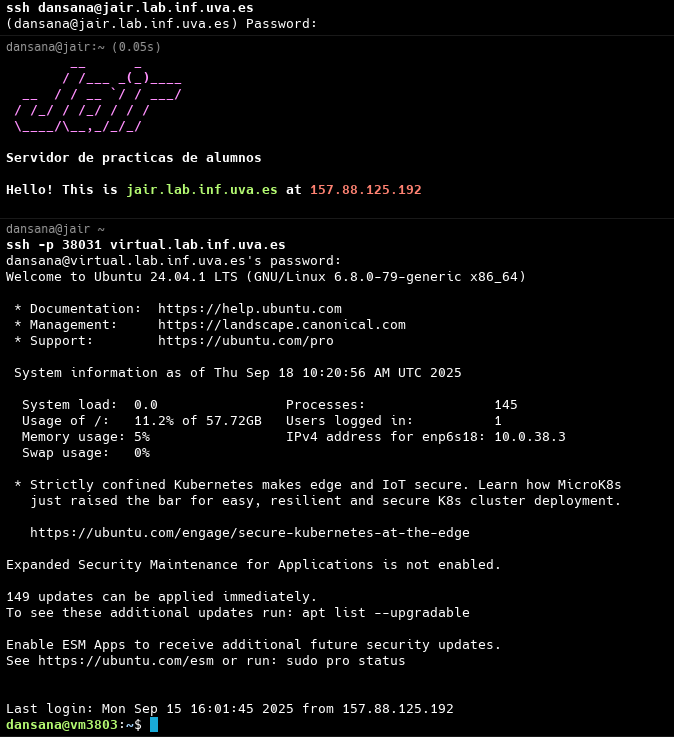
\includegraphics[width=0.6\linewidth]{Recursos/ssh.png}
	\end{figure}
	
	\subsection{Activar cuenta root}
	Lo siguiente que se indica es activar la cuenta \verb|root| cambiando su contraseña mediante \verb|sudo passwd root| e indicando una clave para ese usuario y así poder acceder a la consola directamente como \verb|root|, ya que por defecto no trae ninguna contraseña y puede ser una brecha de seguridad.
	
	\subsection{Administración del disco}
	Se pide obtener información sobre las particiones lógicas y física de nuestra máquina virtual, con ayuda de los comandos que se explican en las transparencias. 
	Y para saber el sistema de ficheros que se está utilizando, tendremos que hacer un \verb|cat| al fichero \verb|/etc/fstab|, que contiene las informaciones que conciernen al montaje de las particiones que hay en el sistema.
	\begin{figure}[H]
		\centering
		\begin{minipage}{0.5\textwidth}
			\centering
			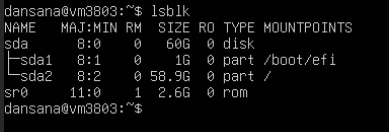
\includegraphics[width=\linewidth]{Recursos/particiones.png}
		\end{minipage}\hfill
		\begin{minipage}{0.45\textwidth}
			\begin{itemize}
				\item \textbf{Dispositivos}: Tal y como se muestra en la imagen, solo tenemos un dispositivo de almacenamiento \verb|sda| con una capacidad de 60G. El otro dispositivo que existe es el CD de instalación de \verb|Ubuntu Server| que ocupa 2.6G.
			\end{itemize}
		\end{minipage}
	\end{figure}
	
	\begin{figure}[H]
		\centering
		\begin{minipage}{0.5\textwidth}
			\centering
			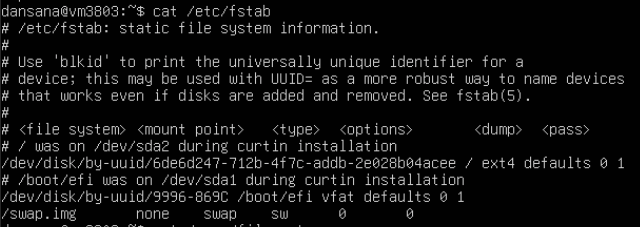
\includegraphics[width=\linewidth]{Recursos/fstab.png}
		\end{minipage}\hfill
		\begin{minipage}{0.45\textwidth}
			\begin{itemize}
				\item \textbf{Particiones}: Existen dos particiones en el disco \verb|sda|:
				\begin{itemize}
					\item \textit{sda1}: Con un tamaño de 1G y montado en el directorio \verb|/boot/efi|, es la encargada de almacenar las herramientas de arranque del sistema que serán lanzadas por el firmware UEFI. Emplea el sistema de ficheros \verb|vfat|.
					\item \textit{sda2}: Partición principal, anclado en el directorio \verb|/|, con el tamaño restante del disco para almacenar todas las aplicaciones y ficheros del sistema operativo y del usuario. Emplea el sistema de ficheros \verb|ext4|.
				\end{itemize}
			\end{itemize}
		\end{minipage}
	\end{figure}
	
	Después, se nos exige investigar el fichero \verb|/proc/filesystems| donde se ubican los sistemas de ficheros que es capaz de entender el sistema.
	\begin{figure}[H]
		\centering
		\begin{minipage}{0.28\textwidth}
			\centering
			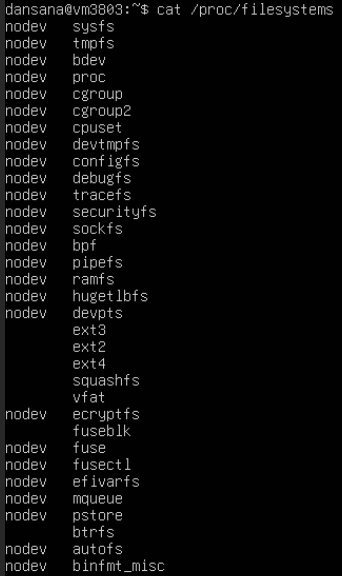
\includegraphics[width=\linewidth]{Recursos/filesystems.png}
		\end{minipage}\hfill
		\begin{minipage}{0.7\textwidth}
			\begin{itemize}
				\item Se muestra dos columnas donde en la izquierda se indica si se requiere un dispositivo de bloque asociado al sistema de fichero que se muestra en la columna de la derecha.
				\item Por ejemplo, para los sistemas de ficheros \verb|ext2, ext3 o ext4| no se indica el valor \verb|nodev|, por lo que es necesario usar un dispositivo físico para usar ese sistema de fichero. Pero, para \verb|tmpfs o proc|, no es necesario tener un dispositivo físico.
			\end{itemize}
		\end{minipage}
	\end{figure}
	
	\subsubsection{Loop} \label{loop}
	Después, creamos un sistema de archivos o fichero dentro de un fichero nuevo:
	\begin{enumerate}
		\item Creamos el fichero mediante el comando \verb|dd|, donde se le indica los siguientes parámetros:\\
		\verb|dd if=/dev/zero of=fichero bs=1 count=4096|
		\begin{itemize}
			\item \textbf{if}: Desde que fichero o directorio se van a leer los datos. Como vamos a crear un fichero vacío, haremos uso de \verb|/dev/zero| que se trata de un fichero especial desde el que se obtiene un flujo de cero, con el propósito de inicializar un fichero.
			\item \textbf{of}: Indicamos la ruta con el nombre del fichero creado. 
			\item \textbf{bs}: Indicamos el tamaño del bloque que se quiere leer y escribir. Para este caso, se escoge de 1 MB por comodidad.
			\item \textbf{count}: El número de bloques que se van a crear. En este caso 4096M que corresponden a los 4G.
		\end{itemize}
		\item El siguiente paso es crear el dispositivo de bloque sobre el fichero que hemos creado con el que trabajaremos para crear el sistema de ficheros, mediante el comando \verb|losetup|:
		\begin{itemize}
			\item Antes de crearlo, tenemos que ver los dispositivos \verb|loop| que están disponibles para asociarlo con el fichero. Para ello, lanzamos el comando \verb|losetup -f| y nos devuelve que el único dispositivo disponible es \verb|/dev/loop0|.
			\item Ahora lo único que tenemos que hacer es ejecutar este comando \verb|sudo losetup /dev/loop0 fichero|. Es necesario usar permisos de administrador, por lo que se lanzará el comando con \verb|sudo|.
		\end{itemize}
		\item Con el dispositivo de tipo bloque, le asignamos un sistema de fichero cualquiera con \verb|mkfs|. En mi caso, le asigno el mismo que el que tiene la partición principal: \verb|sudo mkfs.ext4 /dev/loop0|.
		\item Lo último es montar ese sistema de fichero nuevo en un directorio (\verb|/mnt| debido a que está dedicado a montar dispositivos).
		\item Para comprobar que lo hemos montado correctamente, usamos el comando \verb|lsblk| para ver todas las particiones montadas.
	\end{enumerate}
	\begin{figure}[H]
		\setlength{\abovecaptionskip}{0cm}
		\setlength{\belowcaptionskip}{0cm}
		\centering
		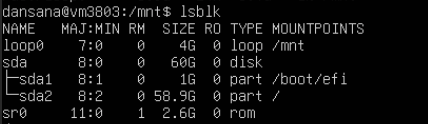
\includegraphics[width=0.6\linewidth]{Recursos/loop0.png}
	\end{figure}
	
	Cuando tengamos el dispositivo de disco \verb|Loop|, nos piden administrar las particiones en ese dispositivo:
	\begin{itemize}
		\item Para crear una partición, haremos uso de la herramienta de \verb|fdisk|. No tendrá ningún valor específico, por lo que se deja todo por defecto.
		\item Puede ser que el kernel no pueda actualizar automáticamente la tabla de particiones al terminar, por lo que habrá que desanclar y volver anclar el \verb|Loop|.
		\item Al igual que hemos hecho con el dispositivo, habrá que formatear esa partición y asignarle un sistema de ficheros. En este caso el mismo que tiene el propio dispositivo.
		\item Después, se monta la partición con el comando \verb|mount| sobre el directorio \verb|/mnt| y se comprueba lanzando un \verb|df -h|. Tras esto, se desmonta con \verb|umount|.
		\item Ahora nos piden un resumen acerca de la función de los ficheros \verb|/etc/fstab| y \verb|/etc/mtab|:
		\begin{itemize}
			\item \textbf{/etc/fstab}: Es un fichero de configuración estático que define qué sistemas de archivos hay en el sistema y cómo deben montarse. La máquina lo consulta durante el arranque para montar automáticamente discos, particiones o sistemas de ficheros de red.
			\item \textbf{/etc/mtab}: Es un fichero dinámico, generado por el sistema, que refleja qué sistemas de ficheros están montados en este momento. En sistemas modernos, muchas veces /etc/mtab es un enlace simbólico a /proc/self/mounts, que cumple la misma función.
		\end{itemize}
		\item Por último, nos indican eliminar la partición existente en \verb|loop0| y crear varias particiones primarias y extendidas o lógicas. Además, cada partición tiene que tener un sistema de ficheros independiente. Este sería el esquema resultante:
		\begin{figure}[H]
			\centering
			\begin{minipage}{0.48\textwidth}
				\centering
				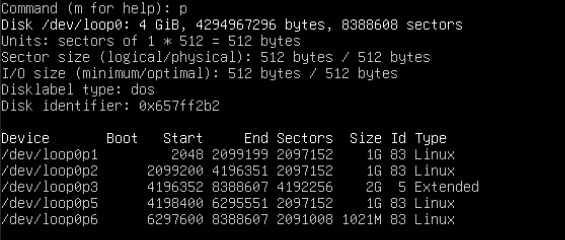
\includegraphics[width=\linewidth]{Recursos/particiones1.png}
			\end{minipage}\hfill
			\begin{minipage}{0.48\textwidth}
				\centering
				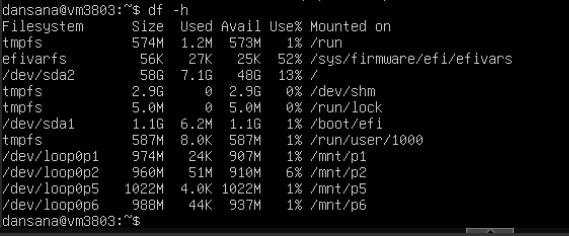
\includegraphics[width=\linewidth]{Recursos/particiones2.png}
			\end{minipage}
		\end{figure}
	\end{itemize}
	
	\subsubsection{LVM}
	Llegados a este punto, se requiere volver a destruir las particiones existentes para crear y administrar volúmenes lógicos (LVM).
	\begin{enumerate}
		\item Primero, modificamos la etiqueta de cada partición para marcar que es de tipo \verb|Linux LVM|. Desde la herramienta de \verb|fdisk|, seleccionamos cada partición del dispositivo \verb|loop0| y con la opción \verb|t|, escogemos el número 44 (en este caso que usamos una tabla de particiones de tipo \verb|GPT|).
		\item Después, creamos el volumen físico en cada partición con \verb|pvcreate|:
		\begin{figure}[H]
			\setlength{\abovecaptionskip}{0cm}
			\setlength{\belowcaptionskip}{0cm}
			\centering
			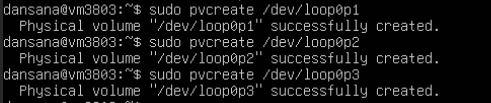
\includegraphics[width=0.6\linewidth]{Recursos/pvcreate.png}
		\end{figure}
		\item Lo siguiente, es crear un grupo de volúmenes físicos, con \verb|vgcreate|, donde agregamos los que hemos creado:
		\begin{figure}[H]
			\setlength{\abovecaptionskip}{0cm}
			\setlength{\belowcaptionskip}{0cm}
			\centering
			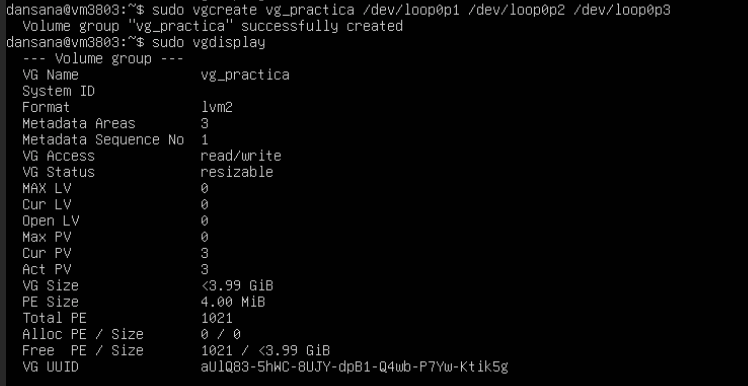
\includegraphics[width=0.6\linewidth]{Recursos/vgcreate.png}
		\end{figure}
		\item Por último, creamos un par de volúmenes lógicos, con \verb|lvcreate|, sobre ese grupo que hemos creado en el punto anterior para después montarlo en el sistema:
		\begin{figure}[H]
			\setlength{\abovecaptionskip}{0cm}
			\setlength{\belowcaptionskip}{0cm}
			\centering
			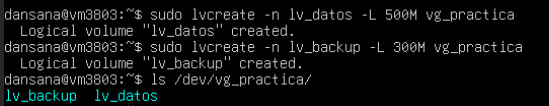
\includegraphics[width=0.6\linewidth]{Recursos/lvcreate.png}
		\end{figure}
		\item Una vez ya tenemos los volúmenes lógicos, los formateamos ambos para asignarles una estructura de directorios y los montamos en el directorio \verb|/mnt| para comprobar que se ha creado de forma correcta:
		\begin{figure}[H]
			\setlength{\abovecaptionskip}{0cm}
			\setlength{\belowcaptionskip}{0cm}
			\centering
			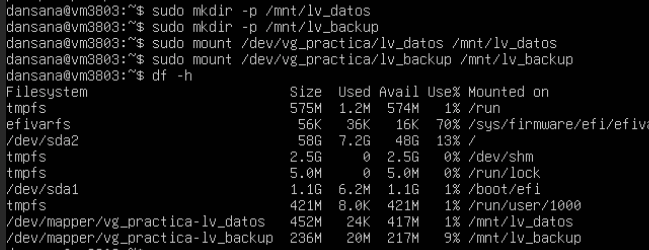
\includegraphics[width=0.6\linewidth]{Recursos/mountLVM.png}
		\end{figure}
		\item Para acabar con este apartado, retornamos el sistema a su estado anterior desmontando y eliminando los volúmenes: 
		\begin{figure}[H]
			\setlength{\abovecaptionskip}{0cm}
			\setlength{\belowcaptionskip}{0cm}
			\centering
			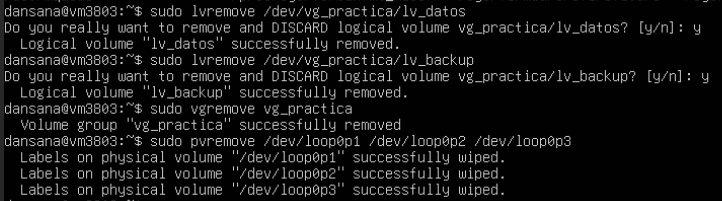
\includegraphics[width=0.6\linewidth]{Recursos/removeLVM.png}
		\end{figure}
	\end{enumerate}
	
	\subsection{Administración de almacenamiento}
	\subsubsection{RAID 5}
	Lo último que vamos a hacer antes de realizar una nueva instalación es crear y administrar un \verb|RAID 5| mediante software:
	\begin{enumerate}
		\item Lo primero es crear 3 nuevos dispositivos \verb|loop| de la misma manera que lo hemos hecho en el apartado \hyperref[sec:loop]{Loop}:
		\begin{figure}[H]
			\setlength{\abovecaptionskip}{0cm}
			\setlength{\belowcaptionskip}{0cm}
			\centering
			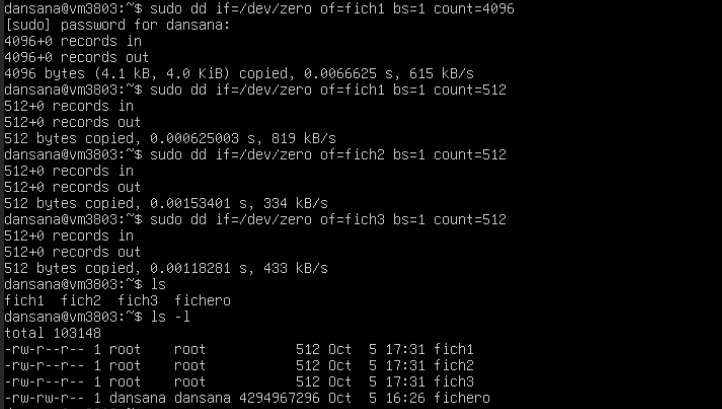
\includegraphics[width=0.6\linewidth]{Recursos/fichRAID.png}
		\end{figure}
		Y después asociarlo a 3 dispositivos \verb|loop|:
		\begin{figure}[H]
			\setlength{\abovecaptionskip}{0cm}
			\setlength{\belowcaptionskip}{0cm}
			\centering
			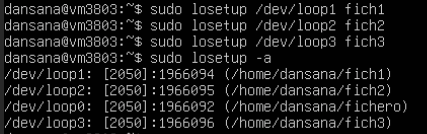
\includegraphics[width=0.7\linewidth]{Recursos/loopRAID.png}
		\end{figure}
		\item Consultando el manual para crear el dispositivo \verb|RAID|, tenemos que seleccionar el modo \verb|Create|, con las opciones de:
		\begin{itemize}
			\item \verb|level|: Indicando el tipo de \verb|RAID|.
			\item \verb|raid-devices|: Número de dispositivos que usaremos.
		\end{itemize}
		\begin{figure}[H]
			\setlength{\abovecaptionskip}{0cm}
			\setlength{\belowcaptionskip}{0cm}
			\centering
			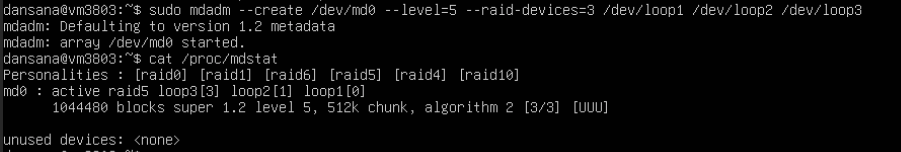
\includegraphics[width=0.9\linewidth]{Recursos/createRAID.png}
		\end{figure}
		\item Ahora repetimos el mismo procedimiento que con el resto de dispositivos de almacenamientos para formatearlos y darle un sistema de ficheros y montarlo:
		\begin{figure}[H]
			\setlength{\abovecaptionskip}{0cm}
			\setlength{\belowcaptionskip}{0cm}
			\centering
			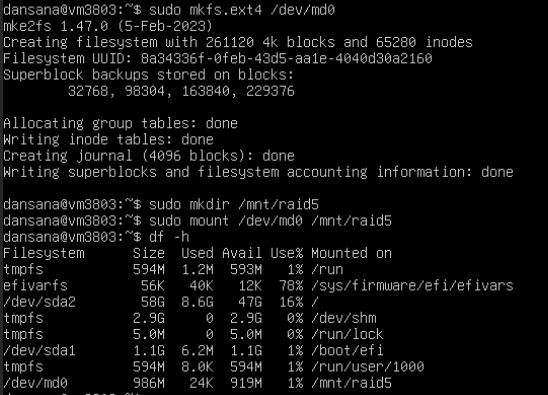
\includegraphics[width=0.6\linewidth]{Recursos/mountRAID.png}
		\end{figure}
	\end{enumerate}
	Para comprobar que hemos configurado correctamente el disco, ejecutamos el comando \\ \verb|echo “Voy a destruir el disco!!!!” > fichero.img| donde \verb|fichero.img| es uno de los ficheros que da soporte al \verb|RAID| para hacerlo fallar y ver que sigue funcionando. Al lanzarlo, veo que no se destruye el disco y sigue activo, debido a que el dispositivo \verb|RAID 5| está montado y funcionando. Entonces, lo que hay que hacer es reiniciar la máquina para que deje de estar en funcionamiento y lanzar el comando. 
	
	\subsection{Nueva instalación personalizada}
	Hasta ahora hemos trabajo con una configuración "por defecto" sobre la administración del disco de la máquina, teniendo únicamente dos particiones: \verb|/boot/efi| empleada para el arranque del sistema y \verb|/| para el resto de archivos del equipo. En un entorno real, tenemos más particiones para minimizar posibles fallos y errores, por lo que vamos a realizar una nueva instalación con las siguientes particiones:
	\begin{itemize}
		\item \verb|/boot/efi|: Contiene los ficheros para el arranque del sistema y tiene un espacio de \verb|1.049G|, que es lo que ocupaba inicialmente y no se puede modificar. El formato que tiene es \verb|fat32|, bastante antiguo y limitado, pero compatible con muchos dispositivos.
		\item \verb|/|: Destinado a todos los ficheros para el sistema operativo y con un espacio de \verb|15G| para que no haya problemas a la hora de agregar elementos al sistema.
		\item \verb|swap|: Con un espacio de \verb|1G|, solo actúa en caso de que la memoria RAM se quede sin espacio. No es necesario añadir nada más ya que el sistema ya cuenta con 6GB de RAM.
		\item \verb|/usr|: Donde se ubica los programas y librerías instaladas, por lo que es necesario \verb|15G| de almacenamiento.
		\item \verb|/var|: Lugar donde se ubican los ficheros como logs y colas. No es necesario dar mucho tamaño, por lo que se le asignan \verb|3GB|.
		\item \verb|/tmp|: Contiene archivos temporales y es necesario separarlo para que en caso de que se ocupe por completo, no bloquee el sistema. Solo es necesario \verb|5G|.
		\item \verb|/home|: Dedicada al espacio personal del usuario que ocupa el resto del espacio restante del disco.
	\end{itemize}
	\begin{figure}[H]
		\setlength{\abovecaptionskip}{0cm}
		\setlength{\belowcaptionskip}{0cm}
		\centering
		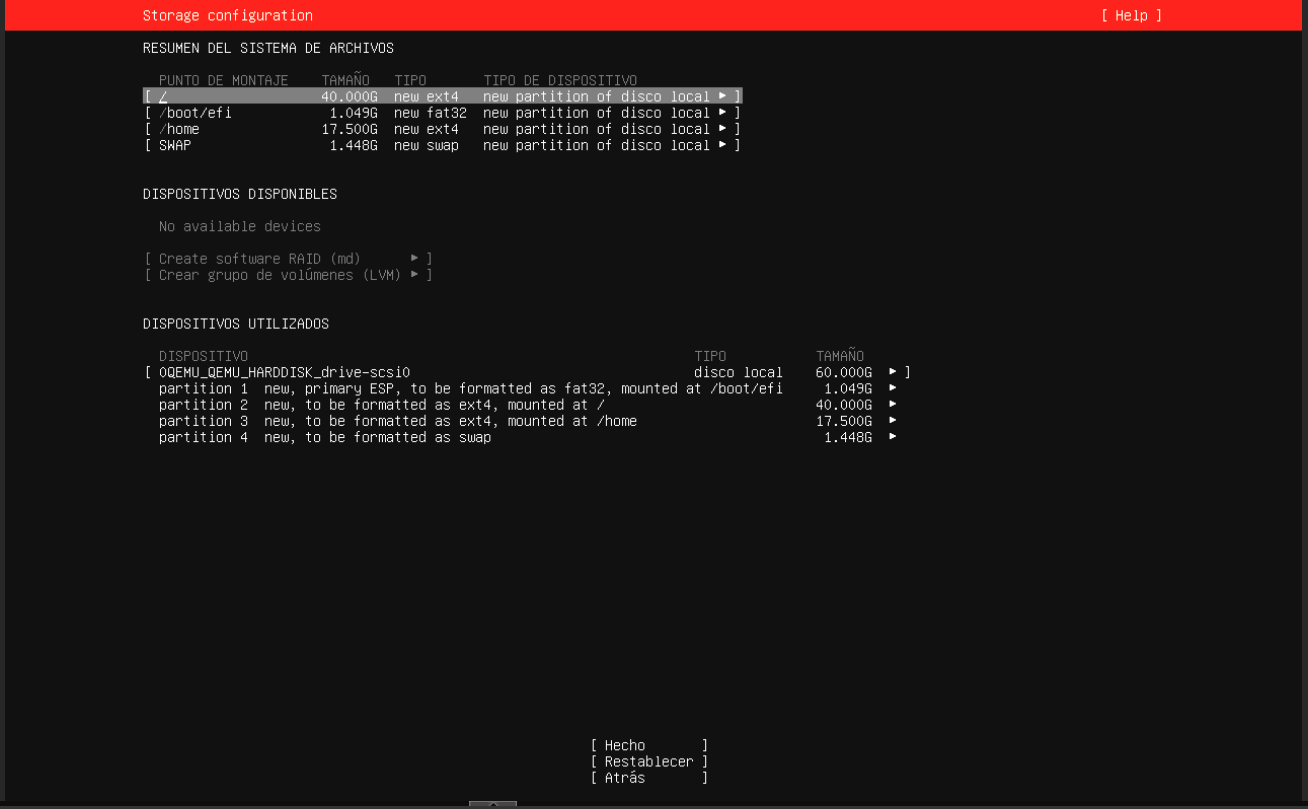
\includegraphics[width=0.6\linewidth]{Recursos/nuevaInstalacion.png}
	\end{figure}
	
	\subsection{Trabajo No Presencial}
	\begin{itemize}
		\item \textbf{Administración de discos – particiones}: 
		\begin{itemize}
			\item Los discos duros o dispositivos de bloques, se dividen en unidades lógicas llamadas \textit{particiones}.\cite{Discos}
			\item Una partición sirve para organizar y almacenar el sistema operativo, las aplicaciones y los archivos personales. Existen diferentes esquemas para la distribución de particiones en un disco, como MBR o GPT.
			\item Cada partición se representa como un archivo en el sistema de archivos de Linux y se encuentra ubicada en el directorio \verb|/dev|.
		\end{itemize}
		\item \textbf{Sistemas de archivos}: 
		\begin{itemize}
			\item Es un elemento que controla cómo se almacenan y recuperan los datos. Sin un sistema de archivos, los datos colocados en un medio de almacenamiento serían un gran cuerpo de datos sin manera de saber dónde termina un dato y comienza el siguiente. 
			\item Se organizan en una estructura jerárquica, de tipo árbol. El nivel más alto del sistema de ficheros es / o directorio raíz. Todos los demás ficheros y directorios están bajo el directorio raíz.\cite{Archivos}
			\item Por debajo del directorio raíz (/) hay un importante grupo de directorios común a la mayoría de las distribuciones de GNU/Linux: \verb|/bin, /boot, /etc/, /opt, etc|.
			\item Tipos de sistemas de ficheros más utilizados en la actualidad:
			\begin{itemize}
				\item \verb|EXT|: Con sus versiones \verb|ext2|, \verb|ext3| y \verb|ext4| (siendo esta la más usada en sistemas Linux), fue creado para sobrepasar las limitaciones de \verb|MINIX| y consiguió implementar \verb|VFS|.
				\item \verb|XFS|: Manejo de grandes volúmenes de datos, por lo que es muy usado en servidores y sistemas empresariales.
				\item \verb|NTFS|: Sistema principal de \verb|Windows| y con cierta compatibilidad con Linux.
				\item \verb|FAT32|: Antiguo y limitado, pero muy compatible con todos los sistemas.
				\item \verb|exFAT|: Evolución del anterior sistema y diseñado especialmente para memorias flash.
			\end{itemize}
		\end{itemize}
		\item \textbf{Actualización de un sistema operativo previamente instalado}:
		\begin{itemize}
			\item En el caso de nuestra máquina virtual, estamos trabajando con \verb|Ubuntu| que pertenece al grupo de distribuciones \verb|Debian|, por lo que para actualizar el sistema operativo una vez instalado se hará uso de la herramienta \verb|apt|.
			\item \verb|apt| nos proporciona un sistema de gestión de paquetes donde maneja automáticamente las dependencias para la instalación de esos paquetes. Requiere de privilegios administrativos.\cite{Actualizar}
			\item Para las actualizaciones será necesario usar los comandos \verb|sudo apt update| y \verb|sudo apt upgrade|.
		\end{itemize}
		\item \textbf{Identificación discos duros y particiones}:
		\begin{itemize}
			\item En Linux, los dispositivos se representan dentro del directorio \verb|/dev| y se identifican como dispositivos de bloques (\verb|sda, sdb, sdc, etc.| o \verb|nvme0n1, nvme0n2, nvme0n3, etc.|).
			\item Además, las particiones, tal y como se mencionaba en el primer apartado, son unidades lógicas de estos dispositivos y se identifican numerándose en orden seguido del nombre del dispositivo (\verb|sda1, sda2, sda3, etc.| o \verb|nvme0n1p1, nvme0n1p2, nvme0n1p3, etc.|).\cite{Discos}
			\item También, cada partición puede tener un \verb|UUID| único, que no cambia aunque el disco se conecte en distinto orden.
		\end{itemize}
		\item \textbf{RAID}: 
		\begin{itemize}
			\item \verb|RAID| o Redundant Array of Independent Disks hace referencia a un sistema de almacenamiento de datos que utiliza múltiples discos duros, entre las cuales se distribuyen o replican los datos. \cite{RAID}
			\item Estas son las principales configuraciones de \verb|RAID|:
			\begin{itemize}
				\item \textbf{RAID 0}: Distribuye los datos equitativamente entre dos o más discos sin información de paridad que proporcione redundancia. No tiene tolerancia a fallos, si falla un disco, lo pierdes todo.
				\item \textbf{RAID 1}: Crea una copia exacta de un conjunto de datos en dos o más discos. Puede fallar solo un disco para no perder todos los datos.
				\item \textbf{RAID 5}: División de datos a nivel de bloques que distribuye la información de paridad entre todos los discos miembros del conjunto. Esta variante de \verb|RAID| ha logrado popularidad gracias a su bajo coste de redundancia. Puede tolerar 1 disco defectuoso; reconstrucción en curso mientras funciona.
				\item \textbf{RAID 6}: amplía el nivel RAID 5 añadiendo otro bloque de paridad, por lo que divide los datos a nivel de bloques y distribuye los dos bloques de paridad entre todos los miembros del conjunto. Puede tolerar 2 discos defectuosos; más seguro que RAID 5 en entornos con discos grandes.
			\end{itemize}
		\end{itemize}
	\end{itemize}
	
	\clearpage
	
	\section{Administración de usuarios y servicios}
	\subsection{Gestión de usuarios y grupos}
	Para comprobar si la clave de nuestro usuario y el resto de usuarios está encriptada, tenemos que ver si en el fichero \verb|/etc/passwd|, dedicado a recopilar la información de un usuario, en el segundo campo aparece escrita la clave o se muestra en su lugar el carácter \verb|'x'|. Con solo lanzar un \verb|cat| a ese fichero, descubrimos que cada usuario tiene su clave encriptada:
	\begin{figure}[H]
		\setlength{\abovecaptionskip}{0cm}
		\setlength{\belowcaptionskip}{0cm}
		\centering
		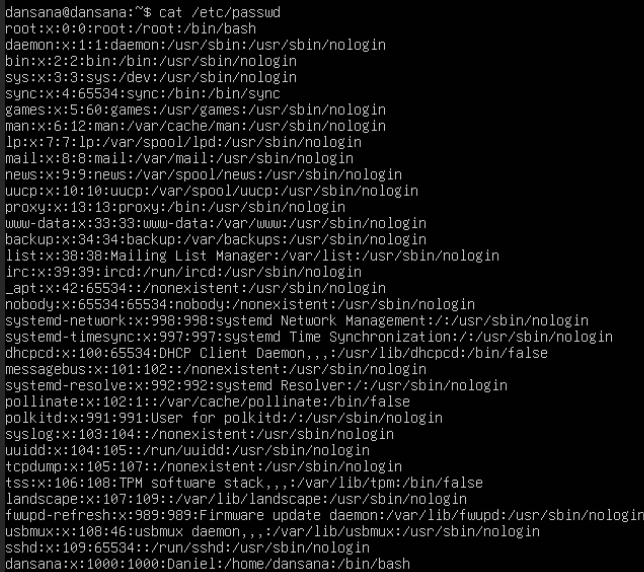
\includegraphics[width=0.6\linewidth]{Recursos/passwd.png}
	\end{figure}
	Con esto concluimos que se está usando el fichero \verb|/etc/shadow| para contener la clave encriptada.\\\\
	Creamos dos nuevos grupos de usuario con \verb|addgroup| y dos usuarios para cada grupo con \verb|useradd|, para crearlos, y \verb|adduser|, para agregarlo a uno de los grupos:
	\begin{figure}[H]
		\centering
		\begin{minipage}{0.48\textwidth}
			\centering
			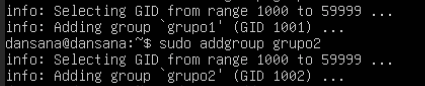
\includegraphics[width=\linewidth]{Recursos/userNuevos.png}
		\end{minipage}\hfill
		\begin{minipage}{0.48\textwidth}
			\centering
			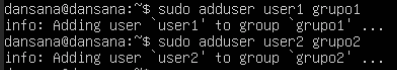
\includegraphics[width=\linewidth]{Recursos/groupNuevos.png}
		\end{minipage}
	\end{figure}
	Tras la creación de los nuevos usuarios y grupos, volvemos a ver el contenido del fichero \verb|/etc/passwd| y también de \verb|/etc/group|, que contiene información de cada grupo y los usuarios que hay dentro de él:
	\begin{figure}[H]
		\centering
		\begin{minipage}{0.48\textwidth}
			\centering
			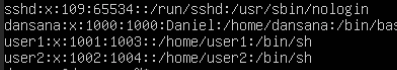
\includegraphics[width=\linewidth]{Recursos/passwdNuevo.png}
		\end{minipage}\hfill
		\begin{minipage}{0.48\textwidth}
			\centering
			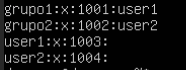
\includegraphics[width=\linewidth]{Recursos/groupNuevo.png}
		\end{minipage}
	\end{figure}
	Y para el \verb|password| de cada usuario, lo recomendable es seguir estos consejos:
	\begin{itemize}
		\item \textbf{Longitud de la contraseña}: Debería haber entre 12 y 16 caracteres.
		\item \textbf{Uso de distintos tipos de caracteres}: Mezclar entre símbolos y letras mayúsculas y minúsculas, incluso números.
		\item \textbf{No utilizar secuencias conocidas}.
	\end{itemize}
	La siguiente tarea es tener una estructura de directorios/ficheros tipo en el directorio \verb|/etc/skel|, encargado de otorgar esa jerarquía al directorio \verb|/home/<user>|. Decidí dar una estructura parecida a la que otorga \verb|Ubuntu Desktop| en su instalación, usando \verb|mkdir|: 
	\begin{itemize}
		\item Downloads
		\item Documents
		\item Images
		\item Desktop
	\end{itemize}
	Al crear otro par de usuarios y agregarlos cada uno a los grupos nuevos, la estructura de ficheros de sus directorios \verb|/home| tendrá esa jerarquía:
	\begin{figure}[H]
		\setlength{\abovecaptionskip}{0cm}
		\setlength{\belowcaptionskip}{0cm}
		\centering
		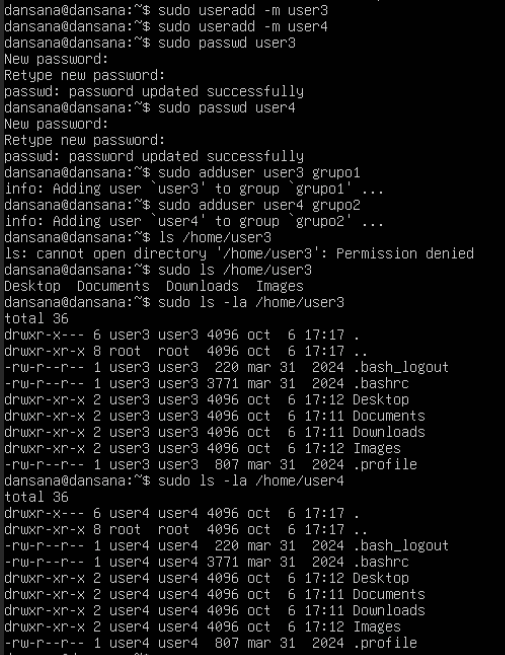
\includegraphics[width=0.6\linewidth]{Recursos/skel.png}
	\end{figure}
	\clearpage
	
	\subsection{Gestión de password}
	Se puede establecer una fecha de caducidad a la contraseña de un usuario y de su cuenta con el comando \verb|chage| que estable dicho atributo. Hay que tener en cuenta que el sistema está 2 horas retrasado de la hora real (se puede comprobar con el comando \verb|date|). Para la contraseña, hay que usar la opción \verb|-M| para indicar el máximo de días que tiene esa contraseña antes de caducar, y la opción \verb|-E| indica la fecha tope de ese usuario:
	\begin{figure}[H]
		\setlength{\abovecaptionskip}{0cm}
		\setlength{\belowcaptionskip}{0cm}
		\centering
		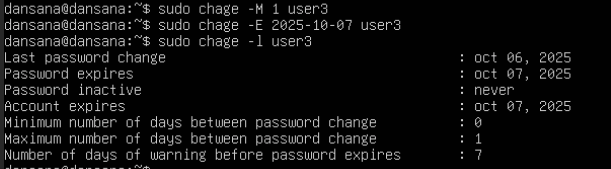
\includegraphics[width=0.7\linewidth]{Recursos/chage.png}
	\end{figure}
	Para comprobar que funciona, podemos verlo en el fichero \verb|/etc/shadow| ya que al tener la información de las claves de los usuarios, se indica también cuando es su fecha de espiración:
	\begin{figure}[H]
		\setlength{\abovecaptionskip}{0cm}
		\setlength{\belowcaptionskip}{0cm}
		\centering
		
\includegraphics[width=\linewidth]{Recursos/shadowChage.png}
	\end{figure}
	
	\subsection{Gestión avanzada de grupos}
	Nos piden que uno de los nuevos usuarios creados forme parte de un de los dos grupos. Compruebo viendo el fichero \verb|/etc/group| que cada usuario está asignado a un grupo, por lo que únicamente habrá usar \verb|usermod| con las opciones \verb|-aG| para añadir a ese usuario a un grupo a mayores. En mi caso lo pruebo con el usuario \verb|user4|.
	\begin{figure}[H]
		\setlength{\abovecaptionskip}{0cm}
		\setlength{\belowcaptionskip}{0cm}
		\centering
		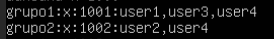
\includegraphics[width=0.6\linewidth]{Recursos/user2group.png}
	\end{figure}
	Una de las ventajas de tener un usuario en varios grupos puede darse a la hora de asignar permisos sobre un recurso compartido, ya que un solo usuario puede tener acceso y privilegios a recursos de ambos grupos.
	\begin{figure}[H]
		\setlength{\abovecaptionskip}{0cm}
		\setlength{\belowcaptionskip}{0cm}
		\centering
		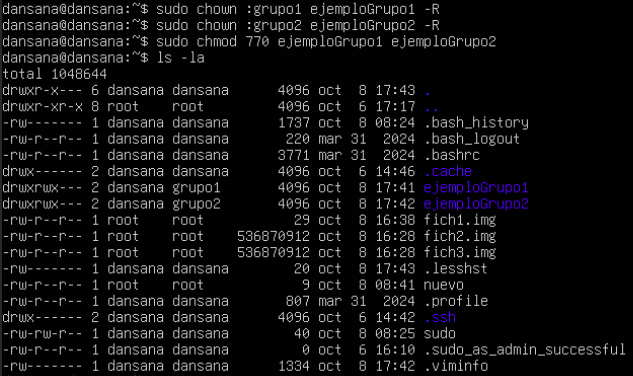
\includegraphics[width=0.7\linewidth]{Recursos/ejemploGroup.png}
	\end{figure}
	
	\subsection{Perfiles de usuario}
	En este apartado, se pide modificar la configuración del editor de texto \verb|vi|, de forma que para uno de los usuarios creados (por ejemplo \verb|user4|) se realicen dos operaciones automáticamente cuando se abra el programa, por lo que será necesario modificar el archivo con la configuración de este editor.\\\\
	Como ya se ha comentado en la instalación, estamos usando \verb|Ubuntu Server 24| en nuestras máquinas virtuales y, consultando la información en foros \cite{rcfile}, en sistemas modernos, utiliza el mismo fichero de configuración que \verb|vim| que es \verb|.vimrc|, porque el comando \verb|vi| es un enlace simbólico al editor \verb|vim|.
	\begin{figure}[H]
		\setlength{\abovecaptionskip}{0cm}
		\setlength{\belowcaptionskip}{0cm}
		\centering
		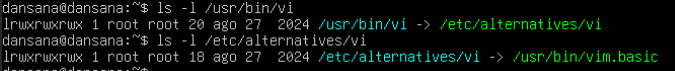
\includegraphics[width=0.8\linewidth]{Recursos/viVim.png}
	\end{figure}
	En \verb|/home/user4|, no existe ese fichero de configuración, por lo que habrá que crearlo y agregar las opciones requeridas.
	\begin{itemize}
		\item Para la auto-sangría, tenemos que activar la opción \verb|autoindent|.
		\item Y para un máximo de 75 caracteres con un salto de línea, la opción \verb|textwidth=75 linebreak|.
	\end{itemize}
	\begin{figure}[H]
		\setlength{\abovecaptionskip}{0cm}
		\setlength{\belowcaptionskip}{0cm}
		\centering
		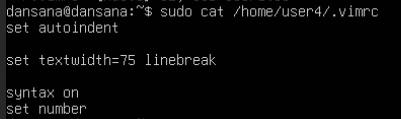
\includegraphics[width=0.8\linewidth]{Recursos/vimrc.png}
	\end{figure}
	Las dos últimas líneas son configuración adicional que he añadido para agregar color al texto y que aparezcan los números de línea por pantalla.
	\begin{figure}[H]
		\setlength{\abovecaptionskip}{0cm}
		\setlength{\belowcaptionskip}{0cm}
		\centering
		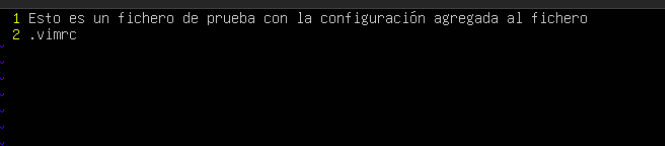
\includegraphics[width=0.8\linewidth]{Recursos/pruebaVi.png}
	\end{figure}
	\clearpage
	
	Finalizado esta primera personalización, ahora nos piden que cada vez que el usuario inicie sesión, se muestre el contenido de \verb|$HOME/docs/Agenda.txt|. Haciendo uso de \verb|Shell scripting|, modificamos el fichero \verb|.profile| porque es el que se ejecuta cuando se inicia sesión en un usuario:
	\begin{figure}[H]
		\setlength{\abovecaptionskip}{0cm}
		\setlength{\belowcaptionskip}{0cm}
		\centering
		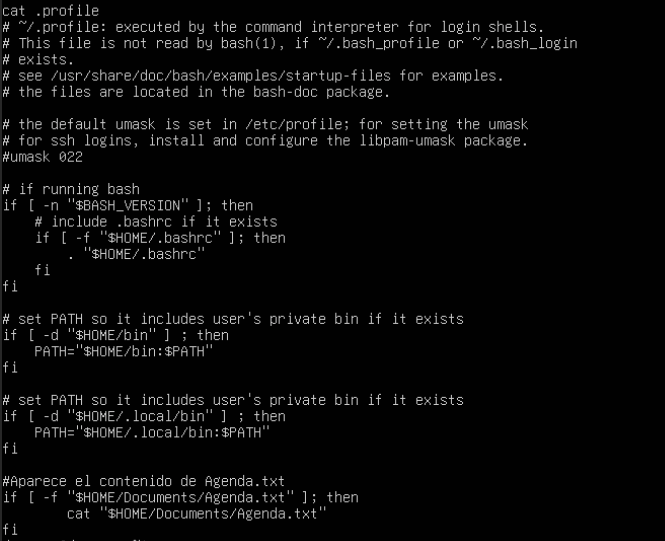
\includegraphics[width=0.7\linewidth]{Recursos/profile.png}
	\end{figure}
	Reiniciando, veremos lo que hay escrito en \verb|Agenda.txt| ubicado en la última línea de todo el contenido que se muestra tras iniciar sesión.
	\begin{figure}[H]
		\setlength{\abovecaptionskip}{0cm}
		\setlength{\belowcaptionskip}{0cm}
		\centering
		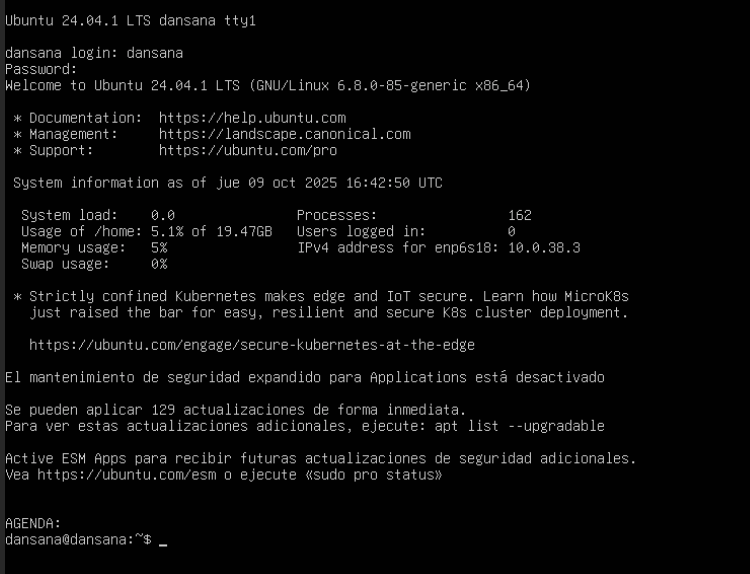
\includegraphics[width=0.7\linewidth]{Recursos/inicioProfile.png}
	\end{figure}
	\clearpage
	
	También, se requiere que cunado el usuario abre un \verb|shell|, se muestre la fecha y hora del último login. En este caso, el fichero \verb|.bashrc| es el que contiene la configuración de cualquier \verb|shell|. Al final del fichero, agregamos \verb|lastlog -u "$USER"| con \verb|tail -n 1|, donde \verb|lastlog| es el comando que muestra el login más reciente de un usuario y \verb|tail| es para mostrar solo la última línea del registro.
	\begin{figure}[H]
		\setlength{\abovecaptionskip}{0cm}
		\setlength{\belowcaptionskip}{0cm}
		\centering
		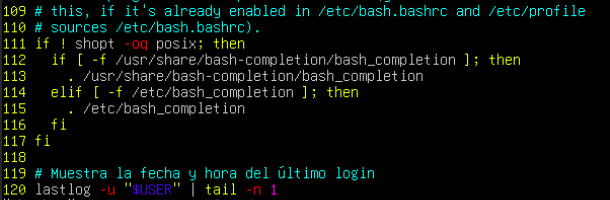
\includegraphics[width=0.7\linewidth]{Recursos/bashrc.png}
	\end{figure}
	Al estar una máquina virtual, no estamos interactuando con una \verb|tty|  "real", por lo que nunca se registrará el inicio de sesión.
	\begin{figure}[H]
		\setlength{\abovecaptionskip}{0cm}
		\setlength{\belowcaptionskip}{0cm}
		\centering
		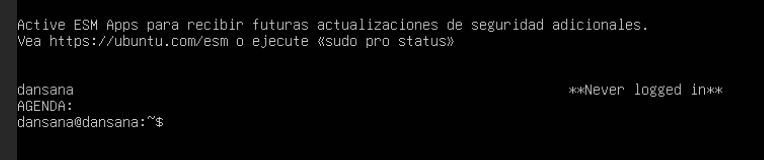
\includegraphics[width=0.7\linewidth]{Recursos/lastlog.png}
	\end{figure}
	Y, finalmente, la última personalización es que cada vez que se cierre sesión, se muestre un mensaje de despedida y solo se cierre sesión tras haber respondido al mensaje. Al hacer \verb|logout|, el sistema ejecuta el fichero \verb|.bash_logout| con todas las instrucciones que contiene. Por ello, modificamos dicho archivo para que mediante un \verb|echo| muestre el mensaje y se quede esperando con un \verb|read|:
	\begin{figure}[H]
		\setlength{\abovecaptionskip}{0cm}
		\setlength{\belowcaptionskip}{0cm}
		\centering
		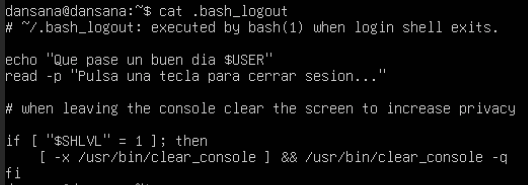
\includegraphics[width=0.7\linewidth]{Recursos/logout.png}
	\end{figure}
	\begin{figure}[H]
		\setlength{\abovecaptionskip}{0cm}
		\setlength{\belowcaptionskip}{0cm}
		\centering
		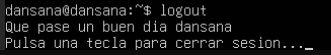
\includegraphics[width=0.7\linewidth]{Recursos/logout1.png}
	\end{figure}
	\clearpage
	
	\subsection{Servicios del sistema}
	En este apartado, se trabajará acerca de los servicios que hay en el sistema, destacando el de conexión segura o \verb|ssh|. Para comprobar los servicios activos, lanzamos el comando \\ \verb|systemctl list-units --type=service --state=running| donde señalamos que en el listado de servicios nos interesa aquellos que están activos:
	\begin{figure}[H]
		\setlength{\abovecaptionskip}{0cm}
		\setlength{\belowcaptionskip}{0cm}
		\centering
		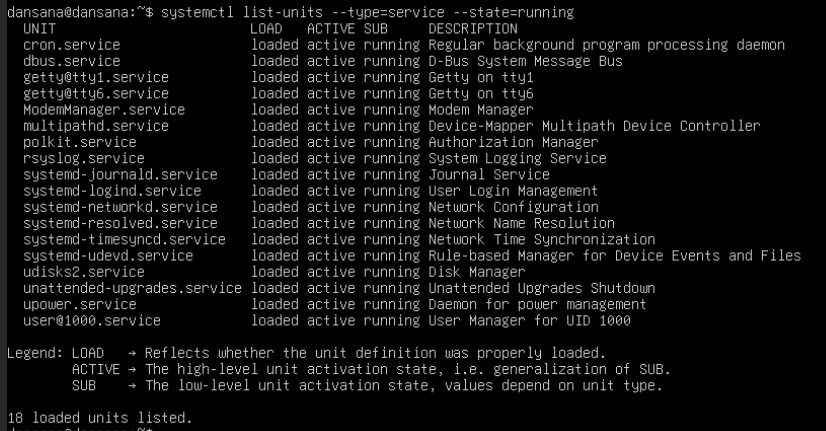
\includegraphics[width=0.7\linewidth]{Recursos/activeProcess.png}
	\end{figure}
	Cada proceso nos indica el nombre (\verb|UNIT|), si está cargado en el sistema (\verb|LOAD|), si está activo (\verb|ACTIVE|), su estado (\verb|SUB|) y una descripción (\verb|DESCRIPTION|). Observando la lista, vemos que no aparece el servicio \verb|ssh| porque está inactivo:
	\begin{figure}[H]
		\setlength{\abovecaptionskip}{0cm}
		\setlength{\belowcaptionskip}{0cm}
		\centering
		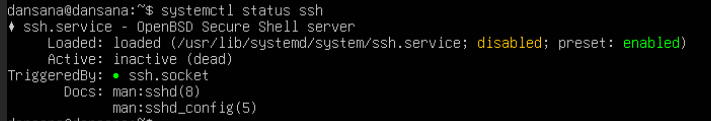
\includegraphics[width=0.8\linewidth]{Recursos/statusSSH.png}
	\end{figure}
	Vemos que está desactivado, por lo que habrá que activarlo con \verb|sudo systemctl enable ssh|, después se para con el mismo comando pero usando \verb|stop| en vez de \verb|enable|, y se iniciará con \verb|start|.
	\begin{figure}[H]
		\setlength{\abovecaptionskip}{0cm}
		\setlength{\belowcaptionskip}{0cm}
		\centering
		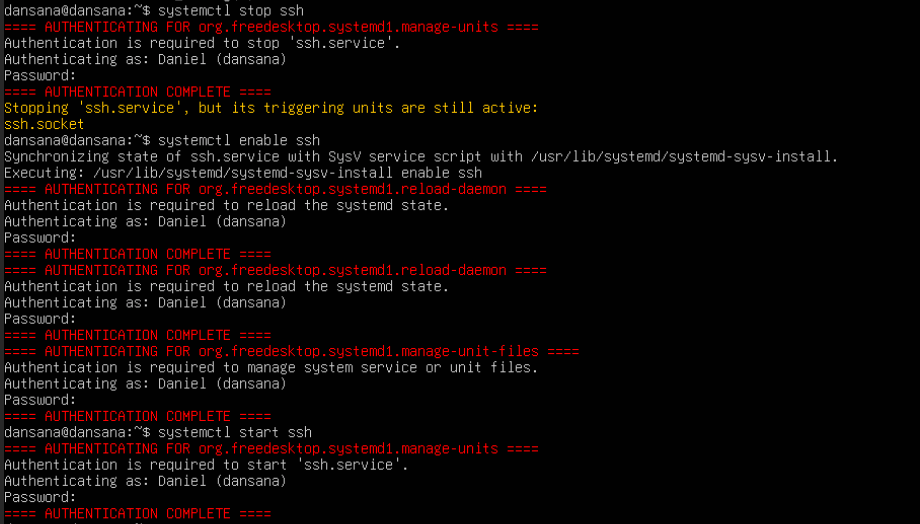
\includegraphics[width=0.7\linewidth]{Recursos/sshService.png}
	\end{figure}
	Es esencial tener un equipo con los servicios esenciales activos y desactivar aquellos que no tienen mucha relevancia, ya que consumen recursos innecesarios y pueden llegar a ser un riesgo en la seguridad. Investigando el listado de servicios que hay activos en mi máquina, hay ciertos servicios que se pueden quitar como \verb|ModemManager.servicie| debido a que solo se emplea para la gestión de módems 3G/4G.\\\\
	Y para terminar con esta sección, nos piden que el sistema desde el arranque vaya al nivel de ejecución 3 (\verb|runlevel3|), es decir sin entorno gráfico y solo en modo texto con red. Dependiendo de cada \verb|runlevel| entre 1 y 5, Linux se ejecutará de una forma distinta. Para arrancar como ese nivel de ejecución \verb|sudo systemctl set-default multi-user.target|
	\begin{figure}[H]
		\setlength{\abovecaptionskip}{0cm}
		\setlength{\belowcaptionskip}{0cm}
		\centering
		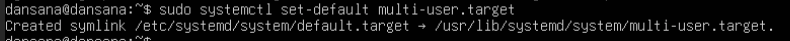
\includegraphics[width=0.9\linewidth]{Recursos/runlevel.png}
	\end{figure}
	
	\subsection{Permisos de acceso}
	Vamos a aprender acerca de cómo funcionan los permisos en sistemas Linux \cite{umask}. En los sistemas operativos tipo \verb|POSIX| cada elemento del sistema de archivos tiene la característica de poseer permisos que lo ubican dentro del mismo. Éstos sirven como uno más de los niveles de seguridad del sistema operativo al impedir que cualquier usuario pueda leer, escribir, ejecutar o acceder a dichos archivos y directorios de manera arbitraria. Estos permisos vistos de manera básica son: lectura (r, \verb|read|), escritura (w, \verb|write|) y ejecución (x, \verb|execution|) y se agrupan en bloques (\verb|rwx|) para 3 diferentes clases (usuario, grupo y otros).\\\\
	Por defecto, cuando se crea un elemento en el sistema de fichero, se le asignará unos permisos dependiendo del objeto creado. \verb|umask| es una función que establece los permisos predeterminados para los nuevos archivos y directorios creados en el sistema. El valor de la máscara de usuario, que se asigna ejecutando \verb|umask|, corresponde a los bits contrarios del permiso predeterminado que se quiera asignar. Es decir, si por ejemplo se quiere asignar una máscara de usuario equivalente a 0775 (\verb|rwxrwxr-x|), el valor de la máscara de usuario corresponderá a 0002 (el resultado de la operación 777 menos 775), que será lo mismo que definir \verb|u=rwx,g=rwx,o=rx|. En este caso, para lograr que cuando se cree un fichero tenga los permisos 550, tenemos que saber que los permisos por defecto son 664 y realizar el siguiente cálculo: \verb|550 = 664 - umask|. El resultado de \verb|umask| es 114 en octal. Para aplicarlo a todos los usuarios, tenemos que agregar al final del fichero \verb|/etc/profile| esta línea \verb|umask 114|.
	\begin{figure}[H]
		\centering
		\begin{minipage}{0.48\textwidth}
			\centering
			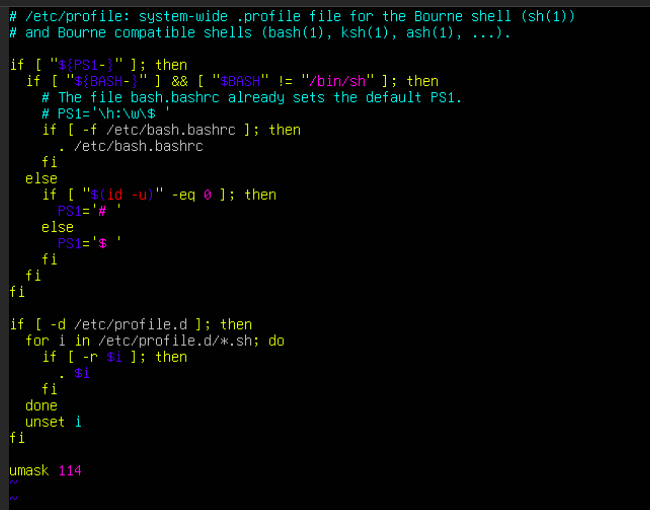
\includegraphics[width=\linewidth]{Recursos/etcProfile.png}
		\end{minipage}\hfill
		\begin{minipage}{0.48\textwidth}
			\centering
			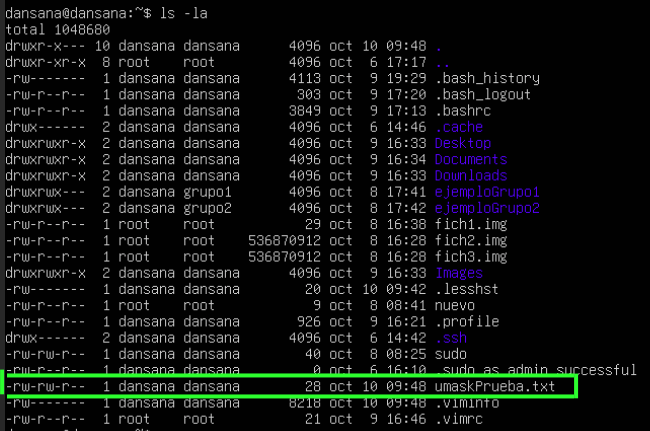
\includegraphics[width=\linewidth]{Recursos/umaskPrueba.png}
		\end{minipage}
	\end{figure}
	\clearpage
	
	Acerca del bit \verb|SetUID|, es un permiso especial que hace que cuando se ha establecido ejecución, el proceso resultante asumirá la identidad del usuario dado en la clase de usuario (propietario del elemento). Corresponde al primer dígito del conjunto octal de permisos de los cuatro que hay. Un ejemplo para ver cómo funciona sería creando un programa en C que me indique cuál es el valor del \verb|UID| efectivo (permisos con los que ejecuta el usuario) y real (permisos de ejecución reales de ese usuario).
	\begin{figure}[H]
		\setlength{\abovecaptionskip}{0cm}
		\setlength{\belowcaptionskip}{0cm}
		\centering
		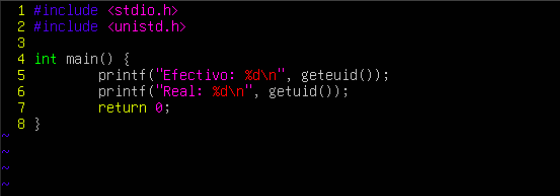
\includegraphics[width=0.9\linewidth]{Recursos/muestraUID.png}
	\end{figure}
	Ahora, le otorgamos permisos a \verb|root| para comprobar cómo varía el valor del \verb|UID|:
	\begin{figure}[H]
		\setlength{\abovecaptionskip}{0cm}
		\setlength{\belowcaptionskip}{0cm}
		\centering
		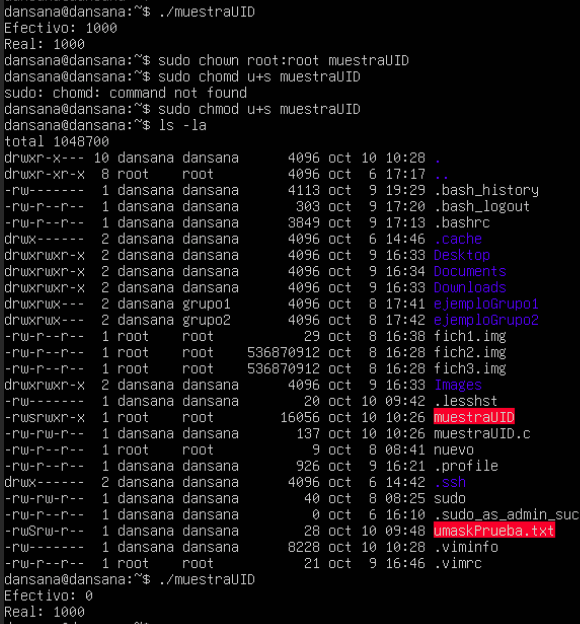
\includegraphics[width=0.7\linewidth]{Recursos/rootUID.png}
	\end{figure}
	
	\subsection{Listas de acceso de control}
	Volvemos a crear dos usuarios nuevos y lo asignamos cada uno a un grupo nuevo distinto, de la misma manera que se ha hecho al comienzo de esta sección. Iniciando sesión en el \verb|userA|, creamos el directorio con solo permisos de lectura y acceso, el cuál va a contener un fichero con solo permiso de lectura para el usuario \verb|root|.\\\\
	Ahora, mediante el uso de la utilidad \verb|ACL|, damos permisos de lectura únicamente al usuario \verb|userB| con el comando \verb|sudo setfacl -m u:userB:r /home/userA/dirNuevo/fichUserA.txt| donde indicamos con la opción \verb|-m| que se quiere modificar la \verb|ACL| del fichero y señalamos el usuario que obtiene esos permisos:
	\begin{figure}[H]
		\setlength{\abovecaptionskip}{0cm}
		\setlength{\belowcaptionskip}{0cm}
		\centering
		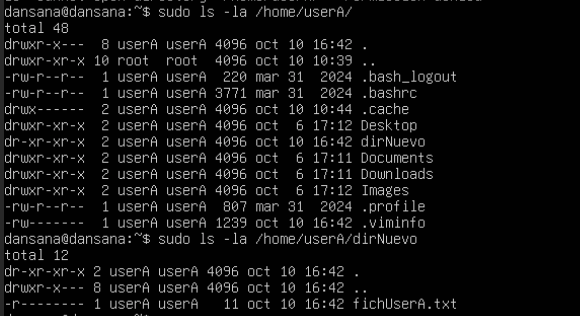
\includegraphics[width=0.7\linewidth]{Recursos/userA.png}
	\end{figure}
	\begin{figure}[H]
		\setlength{\abovecaptionskip}{0cm}
		\setlength{\belowcaptionskip}{0cm}
		\centering
		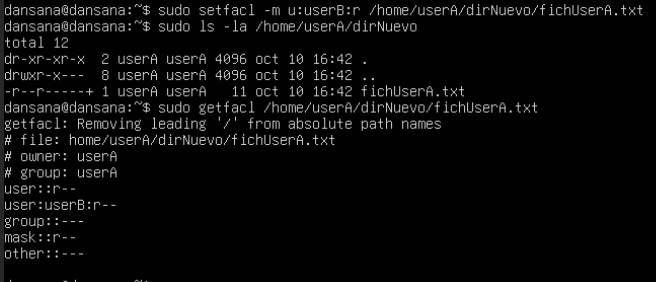
\includegraphics[width=0.7\linewidth]{Recursos/setfaclUserB.png}
	\end{figure}
	\textbf{NOTA}: La utilidad no viene instalada en la máquina, hay que instalarla con \verb|sudo apt install acl|.
	\clearpage
	
	\subsection{Cuota de disco}
	Se trata de un límite establecido por el administrador del sistema que restringe ciertos aspectos del uso del sistema de archivos en los sistemas operativos modernos. El objetivo de la utilización de las cuotas de disco es limitar la asignación de espacio en el disco duro de una manera razonable \cite{quota}. Para activarla, tenemos que seguir estos pasos\cite{disk_quota}:
	\begin{enumerate}
		\item Instalamos la herramienta con el comando \verb|sudo apt install quota|.
		\item Una vez instalada, tenemos que editar el fichero \verb|/etc/fstab|, para activar las opciones de cuota en la partición \verb|/home|, tanto del usuario como para el grupo.
		\begin{figure}[H]
			\setlength{\abovecaptionskip}{0cm}
			\setlength{\belowcaptionskip}{0cm}
			\centering
			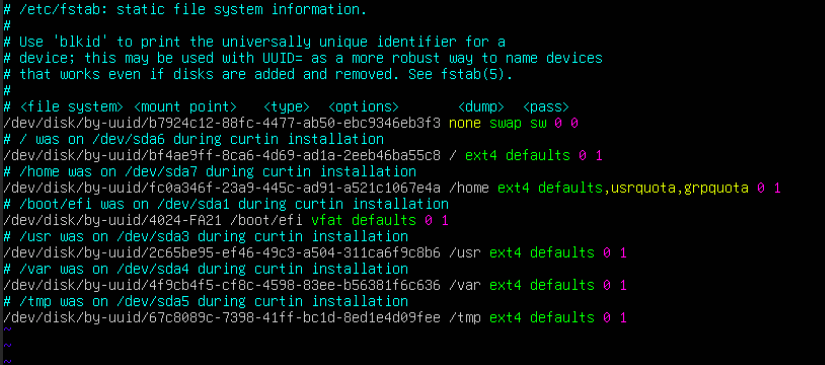
\includegraphics[width=0.7\linewidth]{Recursos/fstabQuota.png}
		\end{figure}
		\item Remontamos la partición con \verb|mount -o remount /home| y reiniciamos los servicios demonios con \\ \verb|sudo systemctl daemon-reload|.
		\item Creamos el fichero con el índice de cuota con \verb|quotacheck -cum /home| y lo activamos con \verb|quotaon -v /home|.
		\begin{figure}[H]
			\setlength{\abovecaptionskip}{0cm}
			\setlength{\belowcaptionskip}{0cm}
			\centering
			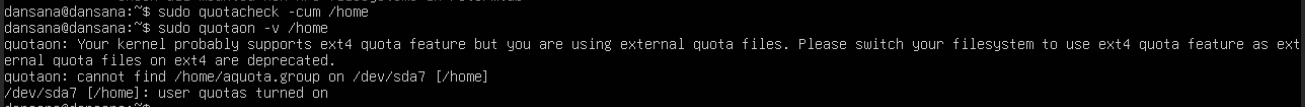
\includegraphics[width=0.9\linewidth]{Recursos/quotaOn.png}
		\end{figure}
		Aparece un mensaje de aviso sobre el tipo de cuotas que puede ser ignorado ya que funciona sin problemas.
		\item Revisamos la configuración de las cuotas de cada usuario con \verb|edquota|, en el que aparece las columnas \verb|soft limit| o límite blando que se puede sobrepasar temporalmente, y \verb|hard limit| o límite duro que indica que no se puede sobrepasar ese límite:
		\begin{figure}[H]
			\setlength{\abovecaptionskip}{0cm}
			\setlength{\belowcaptionskip}{0cm}
			\centering
			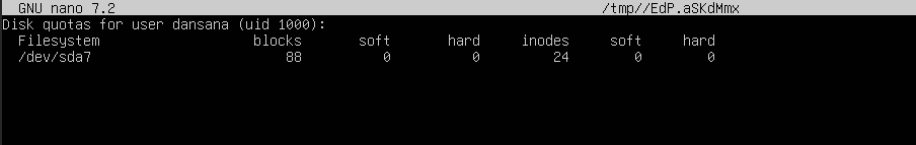
\includegraphics[width=0.9\linewidth]{Recursos/quotaDansana.png}
			\caption{Cuota dansana}
		\end{figure}
	\end{enumerate}
	Un ejemplo donde se puede ver perfectamente su funcionamiento es modificando uno de los ficheros anteriores de los usuarios y estableciendo un límite de cuota tanto duro como blando, y ocupando el espacio disponible hasta ver el mensaje de \verb|Disk quota exceeded|. Para el límite blando, se nos otorga un periodo de 7 días hasta bloquear la escritura en disco.
	
	\subsection{Autoría /tmp}
	La auditoría no proporciona seguridad adicional a su sistema; más bien, puede utilizarse para descubrir violaciones de las políticas de seguridad utilizadas en su sistema. Por ello, para realizar este tipo de operaciones, la herramienta \verb|audit| que nos muestra esta información acerca de cualquier evento:
	\begin{itemize}
		\item Instalamos el servicio con \verb|sudo apt install auditd| y lo arrancamos tal y como hemos visto en el apartado de \verb|Servicios del sistema|.
		\item Después, creamos una nueva regla de auditoría para ese directorio con el comando \\ \verb|sudo auditctl -w /tmp -p rwxa|, donde se indica la carpeta a auditar y las operaciones que se auditan. Comprobamos que se ha agregado correctamente con \verb|sudo auditctl -l|.
		\begin{figure}[H]
			\setlength{\abovecaptionskip}{0cm}
			\setlength{\belowcaptionskip}{0cm}
			\centering
			\includegraphics[width=0.7\linewidth]{Recursos/auditoriaTMP.png}
		\end{figure}
		\item Por último, realizaremos una prueba para ver cuál es contenido del reporte tras crear un fichero en ese directorio y ver su contenido:
		\begin{figure}[H]
			\setlength{\abovecaptionskip}{0cm}
			\setlength{\belowcaptionskip}{0cm}
			\centering
			\includegraphics[width=0.7\linewidth]{Recursos/testAudit.png}
		\end{figure}
		El resultado se puede ver en la última línea, que aparece repetida debido a una comprobación anterior del reporte.
	\end{itemize}
	
	\subsection{Copia de seguridad}
	\subsubsection{dump}
	Consultando el manual, esta herramienta trabaja con sistemas de ficheros \verb|ext2, ext3, ext4| examinado su contenido y determinando qué archivos son necesarios hacer \verb|backup|. Se pueden almacenar tanto en el propio disco como en un medio externo. Después, para recuperar el \verb|backup|, la herramienta que se debe utilizar es \verb|restore| pasando como argumento el fichero \verb|backup|.\\\\
	Existen diferentes opciones a tener en cuenta para realizar la copia de seguridad:
	\begin{itemize}
		\item \textbf{-level}: Nivel de la copia, siendo 0 un copia completo del sistema de ficheros.
		\item \textbf{-f}: El fichero donde queremos tener la copia de seguridad.
		\item \textbf{-u}: Actualiza el historial de copias \verb|/etc/dumpdates|.
		\item \textbf{-z}: Activación del modo compresión de la copia.
	\end{itemize}
	\begin{figure}[H]
		\setlength{\abovecaptionskip}{0cm}
		\setlength{\belowcaptionskip}{0cm}
		\centering
		\includegraphics[width=0.6\linewidth]{Recursos/dump.png}
	\end{figure}
	
	\subsubsection{tar}
	Conocida herramienta para empaquetar y comprimir archivos o directorios en un fichero. Añadir que con el mismo comando podemos también desempaquetar y restaurar los archivos en los discos. Con \verb|tar| podemos preservar los metadatos de los archivos originales, permisos, propiedad o enlaces simbólicos. Esto es muy importante a la hora de realizar copias de seguridad o permitir restaurar los contenidos respetando sus propiedades originales.\\\\
	Las \verb|flags| más utilizadas son las siguientes:
	\begin{itemize}
		\item \textbf{-c}: Indica la creación de un archivo.
		\item \textbf{-v}: Muestra todo lo que se está empaquetando.
		\item \textbf{-f}: Especifica el nombre del archivo comprimido.
		\item \textbf{-x}: Indica que se quiere extraer. 
	\end{itemize}
	\begin{figure}[H]
		\setlength{\abovecaptionskip}{0cm}
		\setlength{\belowcaptionskip}{0cm}
		\centering
		\includegraphics[width=0.9\linewidth]{Recursos/tar.png}
	\end{figure}
	
	\subsubsection{rsync}
	Es una herramienta de sincronización de archivos local y remota, de forma que podemos transferir ficheros de manera eficiente. Utiliza el algoritmo de transferencia delta que minimiza la transferencia de datos al copiar solo las secciones de un archivo que se han actualizado. Admite la copia de enlaces, dispositivos, propietarios, grupos y permisos.\\\\
	Los parámetros más comunes son:
	\begin{itemize}
		\item \textbf{-t}: Indicamos que es de forma recursiva.
		\item \textbf{-a}: Para copiar recursivamente en un directorio, con el añadido de mantener privilegios, permisos y fechas de los ficheros y directorios.
		\item \textbf{-z}: Copiado de forma comprimida.
		\item \textbf{-t}: Preservamos el tiempo de modificación de los archivos.
	\end{itemize}
	\begin{figure}[H]
		\setlength{\abovecaptionskip}{0cm}
		\setlength{\belowcaptionskip}{0cm}
		\centering
		\includegraphics[width=0.9\linewidth]{Recursos/rsync.png}
	\end{figure}
	\clearpage
	
	\section{Autenticación. Seguridad. Control de Servicios.}
	\subsection{PAM}
	En Linux, la autenticación de los usuarios en el sistema está estandarizado mediante el uso de \verb|PAM|. Proporciona un mecanismo para añadir autenticación a los programas mediante el uso de llamadas a las bibliotecas de funciones \verb|PAM|.\\
	El uso de diferentes módulos para cada servicio facilita que cada uno de ellos no tenga que implementar el mecanismo de acceso, sino simplemente pasar las credenciales a \verb|PAM| y este se encargue de indicar si el usuario tiene acceso a no.
	
	\subsubsection{Claves fuertes}
	El comando \verb|passwd| es uno de los que sí usan \verb|PAM| a la hora de crear las contraseñas, ya que en vez comunicarse con los ficheros \verb|/etc/passwd| y \verb|/etc/shadow|, hace una llamada al sistema \verb|PAM| y recibe las instrucciones del fichero \verb|/etc/pam.d/password|, donde realmente tiene su configuración en \verb|/etc/pam.d/common-password|. Comprendido esto, modificaremos este fichero para obligar a los nuevos usuarios a que la nueva contraseña que asignen tenga estos criterios:
	\begin{itemize}
		\item Permitir que, en caso de fallo, sólo reintente 2 veces.
		\item Obligatoriedad de contener al menos 1 carácter numérico, 1 carácter mayúscula y 1 carácter minúscula.
		\item Que no se utilicen palabras claves ya usadas, o que estén en un diccionario.
	\end{itemize}
	Antes de comenzar, \textbf{IMPORTANTE} hacer copia del fichero \verb|/etc/pam.d/password| porque si se comenten errores se puede bloquear los cambios de clave y habrá que formatear la máquina. También, es conveniente tener una sesión \verb|root| abierta en caso de problemas.\\\\
	Este sería el fichero \verb|/etc/pam.d/common-password| actualizado para conseguir cumplir esos criterios:
	\begin{figure}[H]
		\centering
		\begin{minipage}{0.6\textwidth}
			\centering
			\includegraphics[width=\linewidth]{Recursos/common-password.png}
		\end{minipage}\hfill
		\begin{minipage}{0.35\textwidth}
			\begin{itemize}
				\item En el primer módulo, \verb|libpam-pwquality|, indicamos el número de reintentos que tiene el usuario al cambiar la clave y cómo tiene que ser esa clave.
				\item En el segundo módulo, \verb|libpam-pwhistory|, conseguimos que se almacene las 5 últimas contraseñas.
			\end{itemize}
		\end{minipage}
	\end{figure}
	
	\textit{NOTA}: En el caso de perder o dañar dicho archivo y sí tener \verb|backup|, habrá que reiniciar la máquina virtual e ir al CD de \verb|Ubuntu Server| y desde el shell recuperar el fichero.
	
	\clearpage
	
	\subsubsection{Control de acceso por hora y por terminal}
	Siguiendo con el servicio \verb|PAM|, procedemos a cambiar el \verb|login| de nuestra máquina para agregar las siguientes restricciones, a través del fichero \verb|/etc/security/time.conf| que configura las reglas del módulo \verb|pam_time| encargado de la autenticación de un usuario en el sistema:
	\begin{itemize}
		\item Un usuario cualquiera (por ejemplo \verb|userA|) no pueda trabajar de 11:30h a 11:40h.
		\item Que ese mismo usuario no se pueda conectar a la consola.
		\item Y además, pueda acceder al resto de consolas que no sea la \verb|tty1|.
	\end{itemize}
	
	En el fichero, cada línea tiene que tener esta estructura: \verb|services;ttys;users;times|. \\\\ \textbf{IMPORTANTE}: Al igual que antes, hay que hacer copia de los ficheros que vayamos a cambiar en caso de fallo.
	\begin{figure}[H]
		\setlength{\abovecaptionskip}{0cm}
		\setlength{\belowcaptionskip}{0cm}
		\centering
		\includegraphics[width=0.9\linewidth]{Recursos/timeConf.png}
	\end{figure}
	
	\subsection{Crontabd y atd}
	\subsubsection{Crontabd}
	Se trata de un servicio demonio que permite programar tareas automáticas para que se ejecuten de forma periódica. Para asignar un nueva tarea, lanzamos el comando \verb|crontab -e| donde indicamos primero cada cuanto se va a lanzar el script.
	\begin{figure}[H]
		\setlength{\abovecaptionskip}{0cm}
		\setlength{\belowcaptionskip}{0cm}
		\centering
		\includegraphics[width=0.7\linewidth]{Recursos/crontab.png}
	\end{figure}
	
	\subsubsection{atd}
	La orden \verb|at| ejecuta un programa en un momento específico en el futuro. Toma el tiempo y la fecha deseados como parámetros de línea de comandos, y el comando a ejecutar en su entrada estándar. Ejecutará el programa como si hubiese ingresado en la consola.
	\begin{figure}[H]
		\setlength{\abovecaptionskip}{0cm}
		\setlength{\belowcaptionskip}{0cm}
		\centering
		\includegraphics[width=0.7\linewidth]{Recursos/at.png}
	\end{figure}
	
	\subsection{Seguimiento de la ejecución de servicios}
	Para ver los resultados el servicio demonio \verb|crond| en el registro \verb|rsyslogd|, hay que activar el registro y editar su configuración añadiendo la regla de que los \verb|logs| del servicio aparezcan en el registro. La línea que hay que añadir es \verb|cron.*	/var/log/cron.log| y reiniciar tanto el servicio \verb|cron| y el \verb|rsyslog|.
	
	\clearpage
	
	\bibliographystyle{plain}
	\bibliography{bibliografia}
\end{document}